\chapter{Formulario sobre jugadores}
\label{FormularioJugadores}
En este apéndice que muestran las preguntas propuestas en el formulario de estudio de los jugadores\footnote{Como se mencionó en el capítulo 4, en el contexto de la gamificación es más apropiado referirse a los usuarios como \textit{jugadores}} junto con las respuestas obtenidas. El formulatio fue realizado y compartido como un documento \textit{Google Form} para el que no era necesario iniciar sesión o registrarse.

En total, el formulario fue respondido por 12 usuarios diferentes. El formulario se compartió en el grupo de la asignatura de Programación Competitiva de la Facultad de Informática de la Universidad Complutense de Madrid, aunque se instó a los encuestados a compartirlo con otras personas de interés, por lo que no se puede asegurar que todas las respuestas procedan de estudiantes de la asignatura mencionada.

Las preguntas del formulario están dirigidas a saber: cuál es el tipo de jugador para el que estamos diseñando (siguiendo la taxonomía de jugadores propuesta por \cite{bartle_players_muds}), qué uso hacen los encuestados de jueces en línea, y qué tipo de funcionalidades buscan estos jugadores.

\section{Perfil del jugador}

 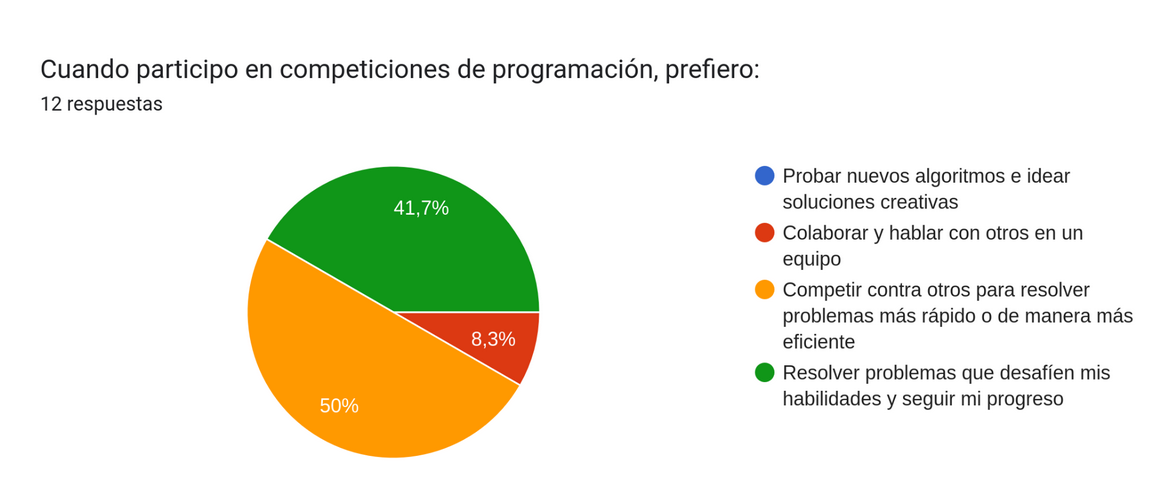
\includegraphics[width=1\textwidth]{Imagenes/Bitmap/ApendiceB/1.png}
 
 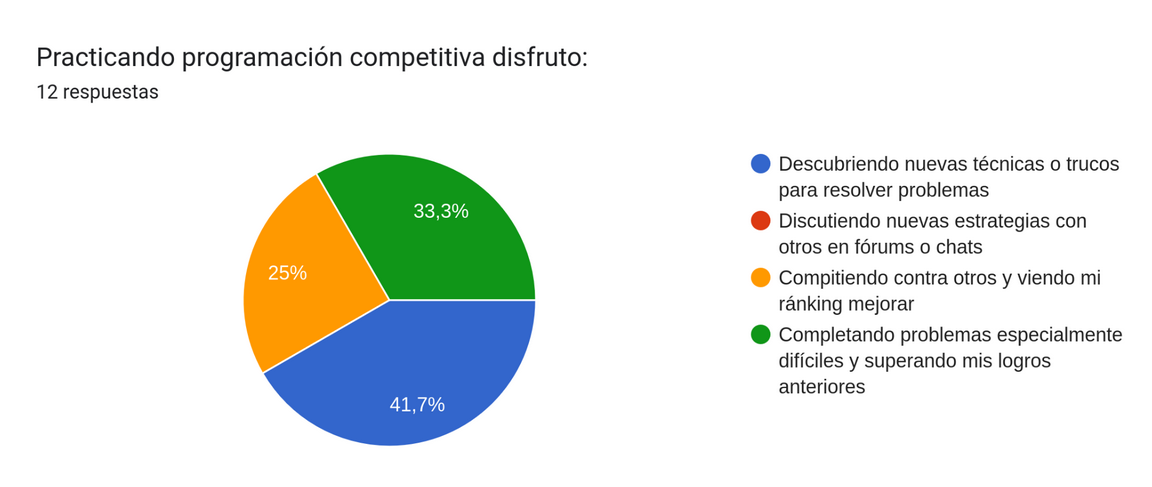
\includegraphics[width=1\textwidth]{Imagenes/Bitmap/ApendiceB/2.png}
 
 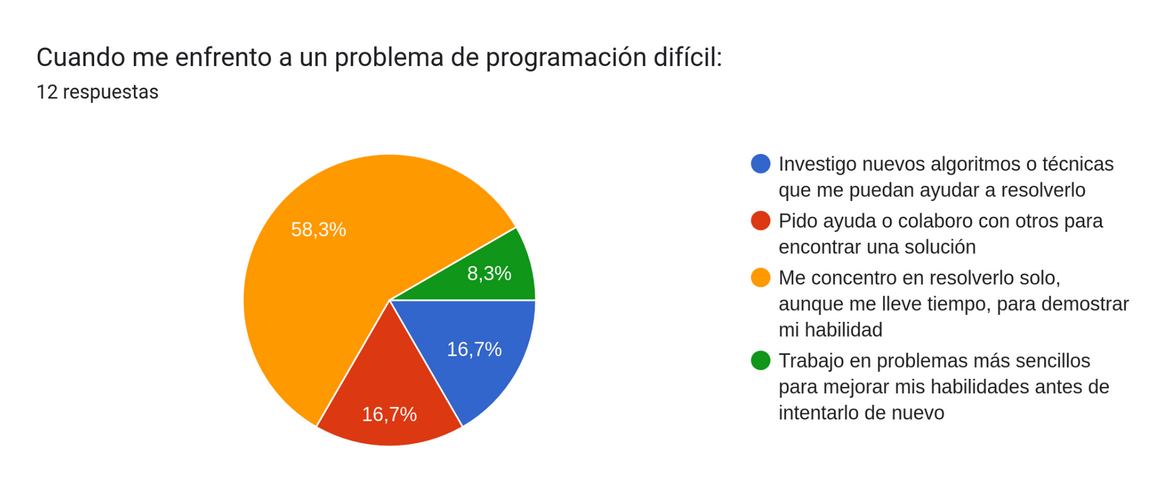
\includegraphics[width=1\textwidth]{Imagenes/Bitmap/ApendiceB/3.png}
 
 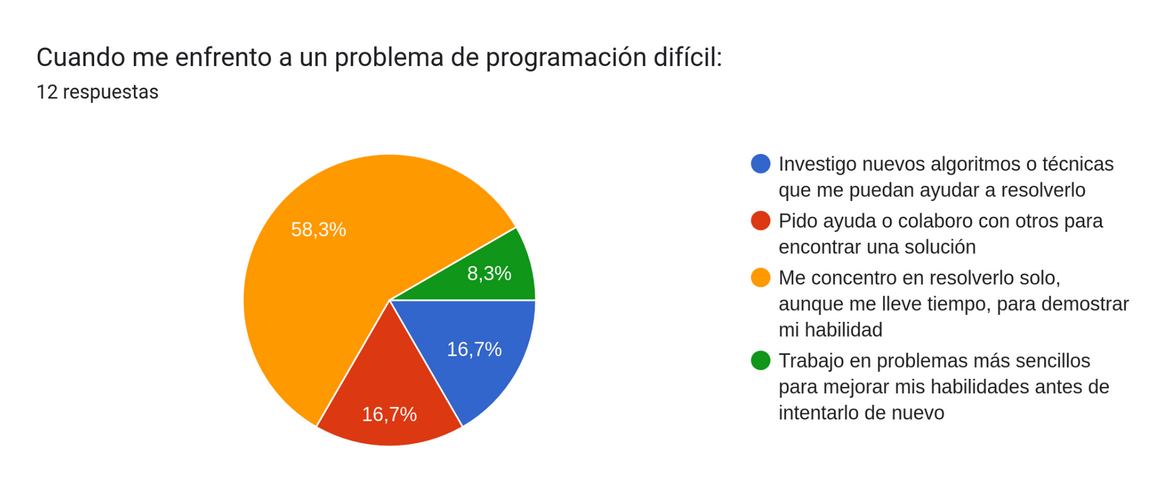
\includegraphics[width=1\textwidth]{Imagenes/Bitmap/ApendiceB/3.png}
 
 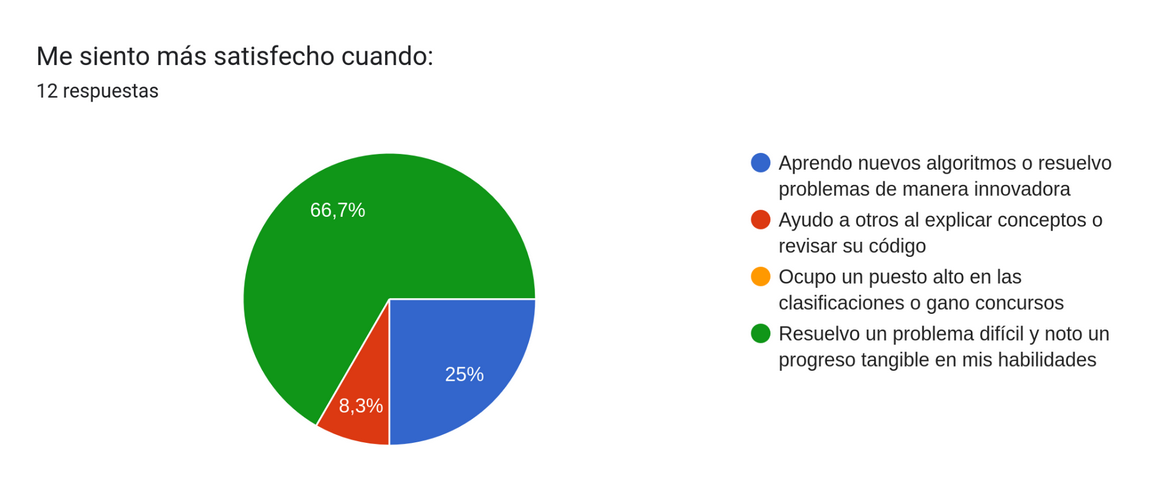
\includegraphics[width=1\textwidth]{Imagenes/Bitmap/ApendiceB/4.png}
 
 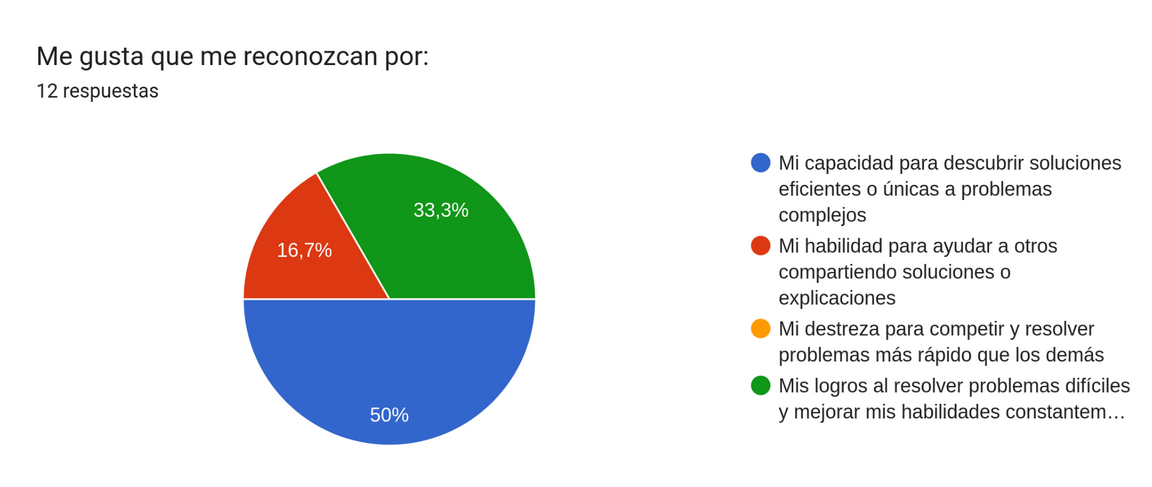
\includegraphics[width=1\textwidth]{Imagenes/Bitmap/ApendiceB/5.png}
 
 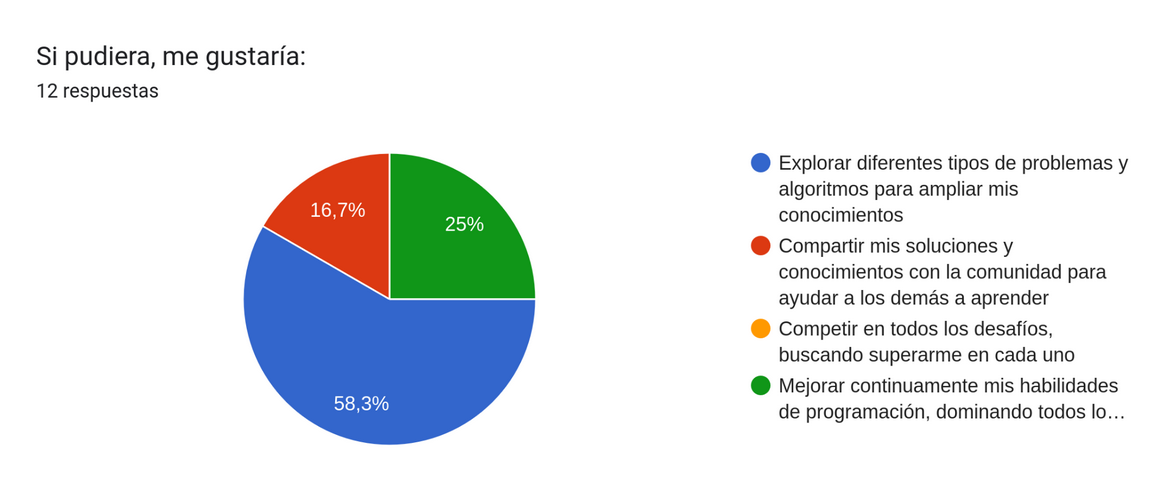
\includegraphics[width=1\textwidth]{Imagenes/Bitmap/ApendiceB/6.png}
 
 \section{Uso de jueces en línea}
 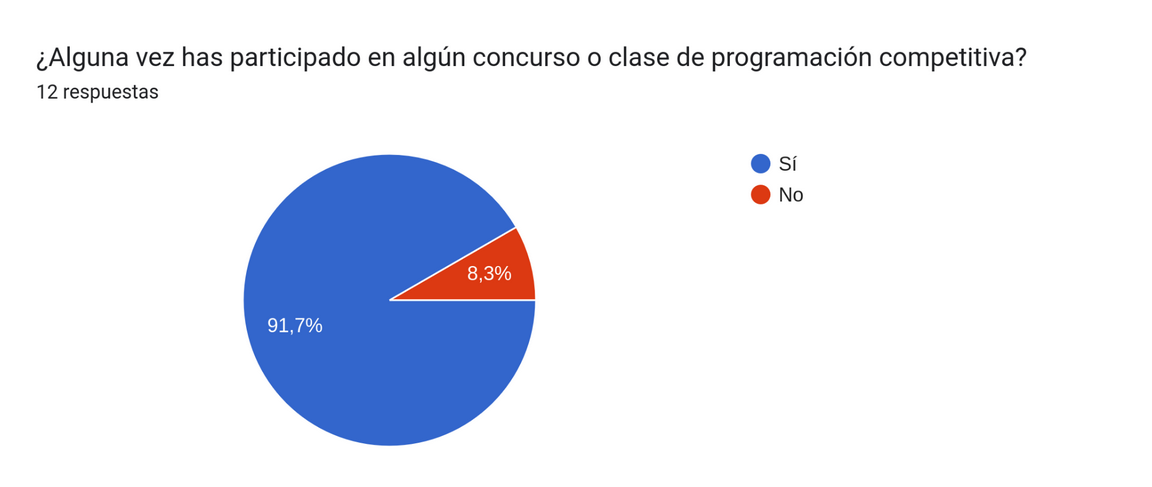
\includegraphics[width=1\textwidth]{Imagenes/Bitmap/ApendiceB/7.png}
 
  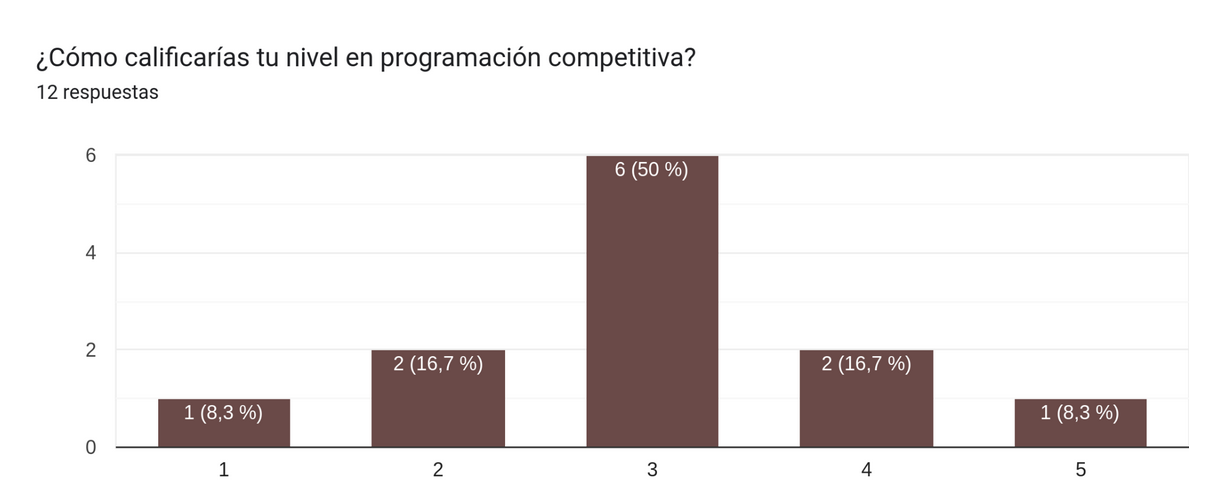
\includegraphics[width=1\textwidth]{Imagenes/Bitmap/ApendiceB/8.png}
  
   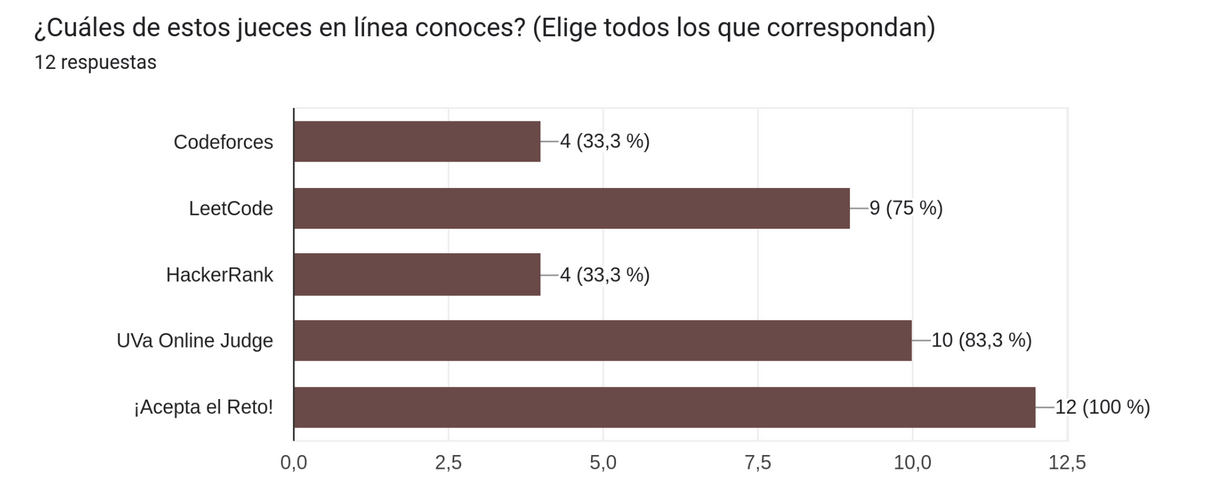
\includegraphics[width=1\textwidth]{Imagenes/Bitmap/ApendiceB/9.png}
   
    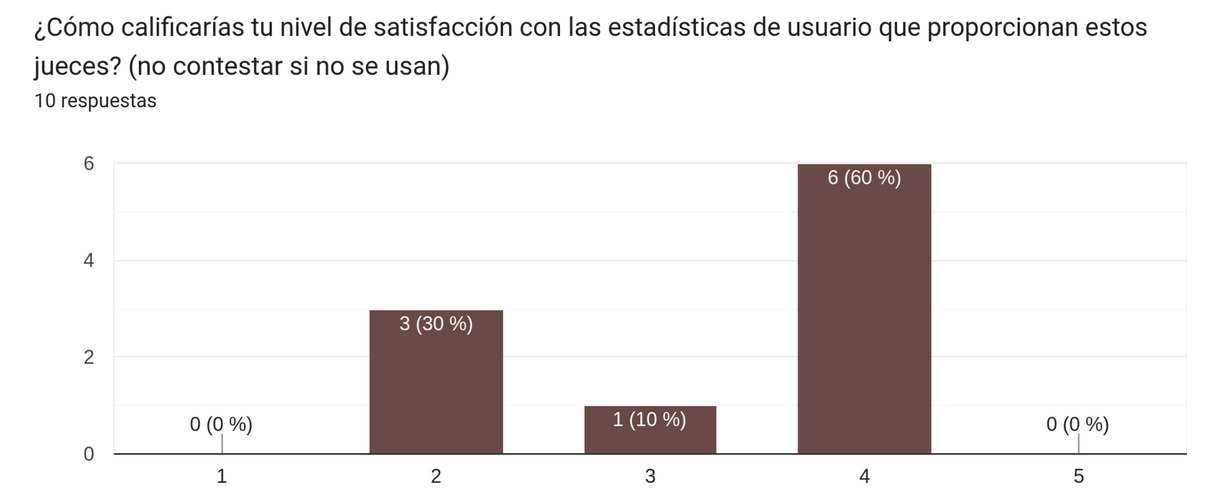
\includegraphics[width=1\textwidth]{Imagenes/Bitmap/ApendiceB/10.png}
    
     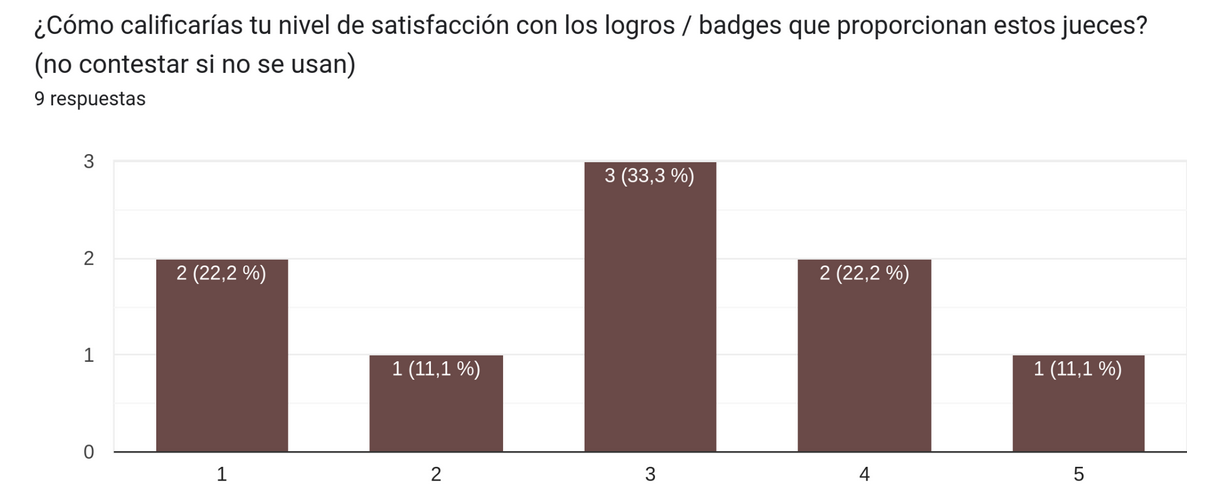
\includegraphics[width=1\textwidth]{Imagenes/Bitmap/ApendiceB/11.png}
     
      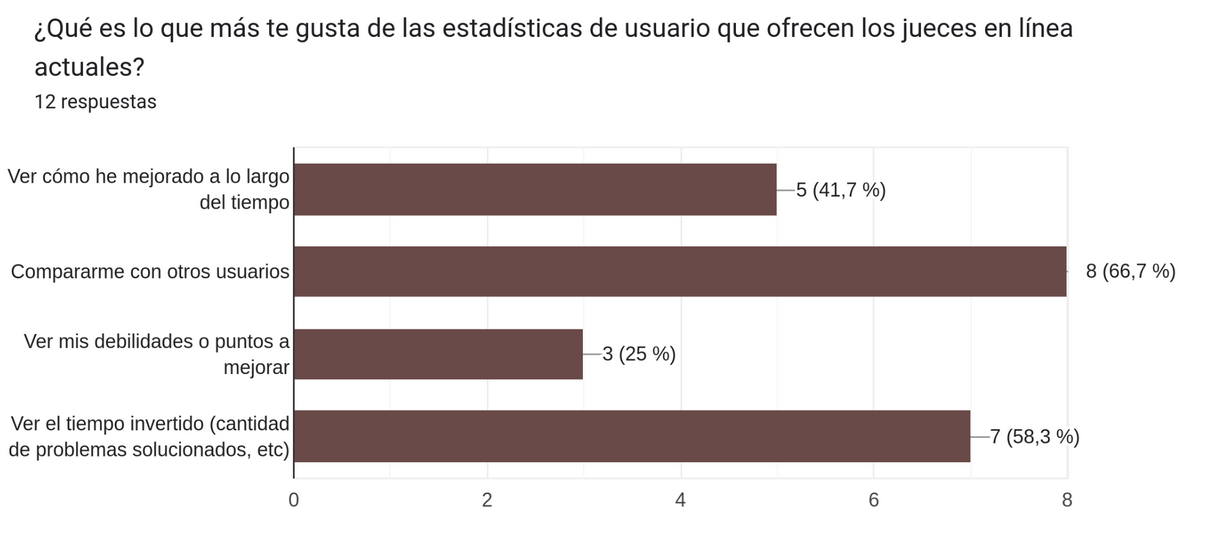
\includegraphics[width=1\textwidth]{Imagenes/Bitmap/ApendiceB/12.png}
      
       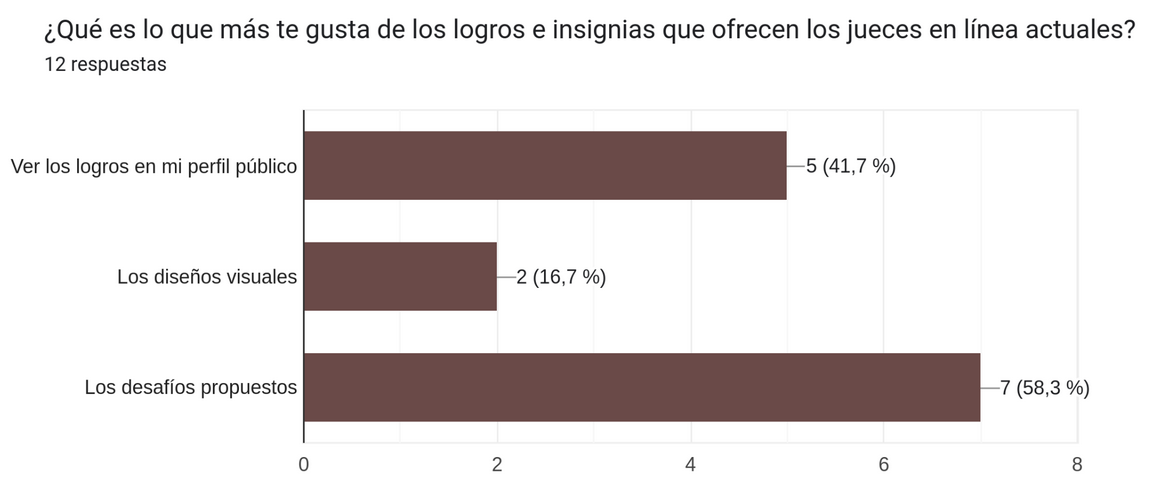
\includegraphics[width=1\textwidth]{Imagenes/Bitmap/ApendiceB/13.png}
       
        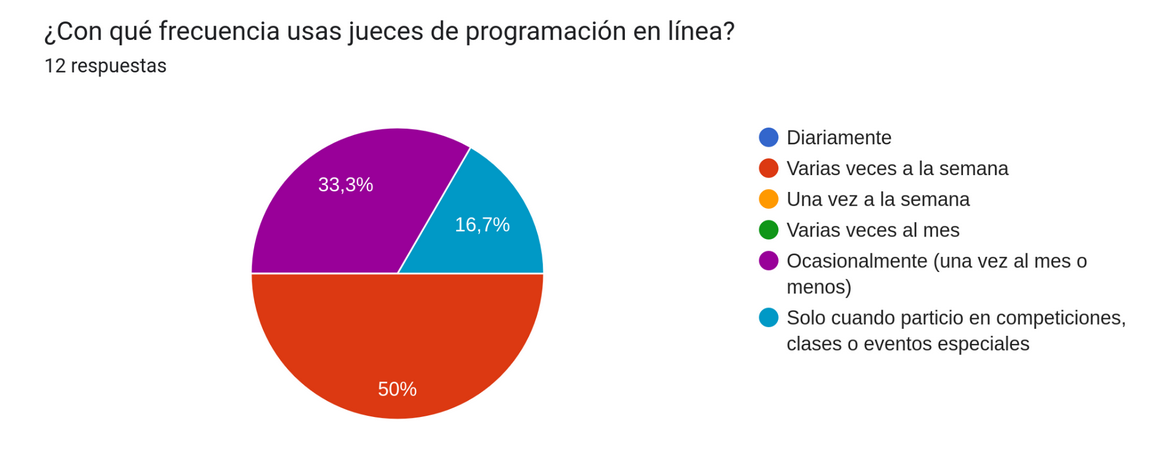
\includegraphics[width=1\textwidth]{Imagenes/Bitmap/ApendiceB/14.png}
        
         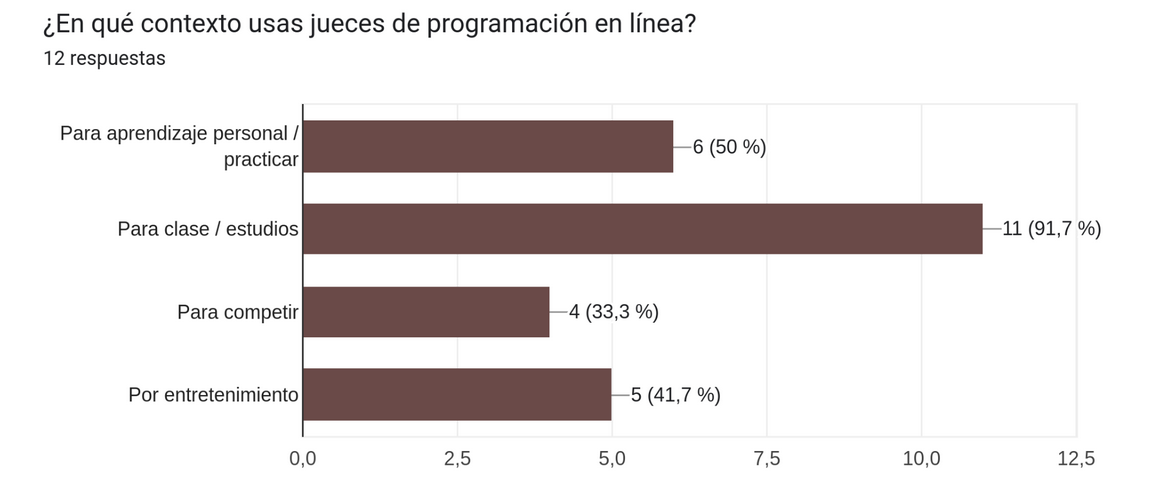
\includegraphics[width=1\textwidth]{Imagenes/Bitmap/ApendiceB/15.png}
         
          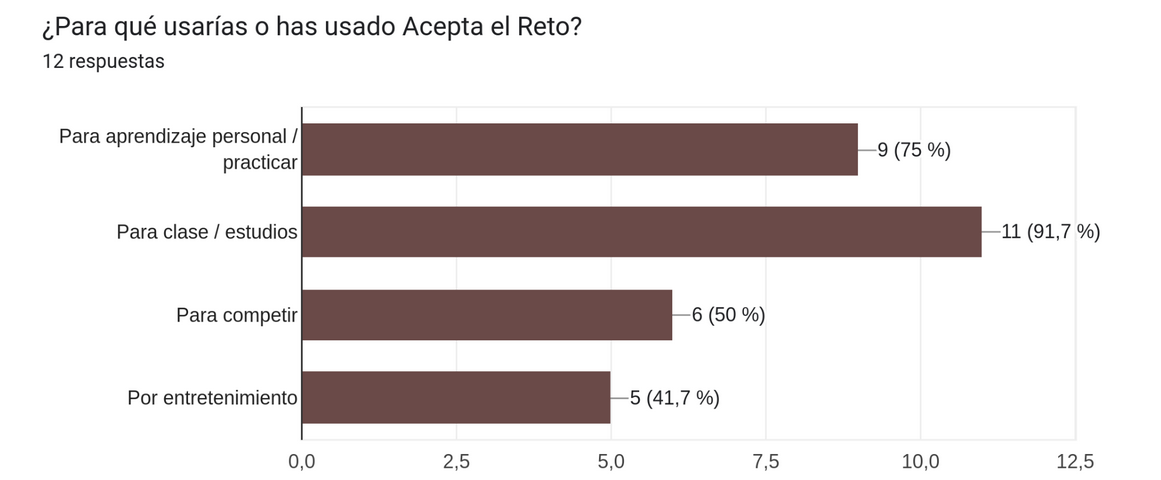
\includegraphics[width=1\textwidth]{Imagenes/Bitmap/ApendiceB/16.png}
          


 \section{Preferencias de recompensas y motivaciones}

           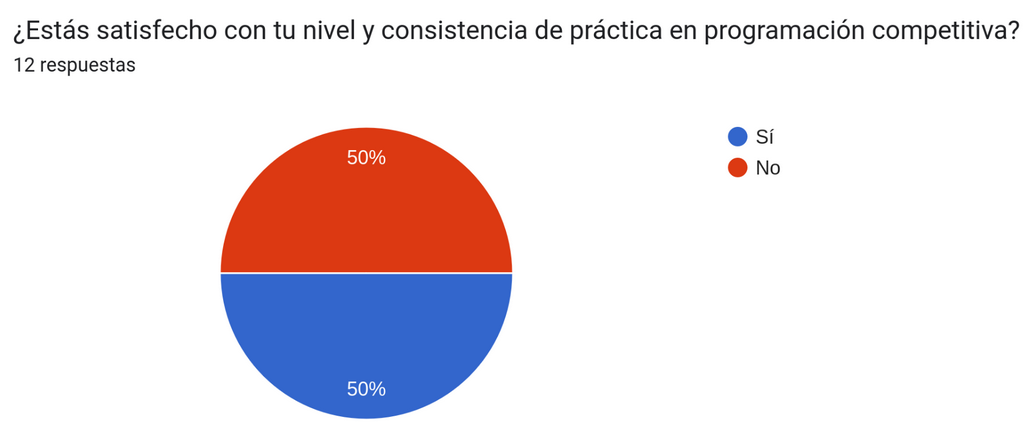
\includegraphics[width=1\textwidth]{Imagenes/Bitmap/ApendiceB/17.png}

          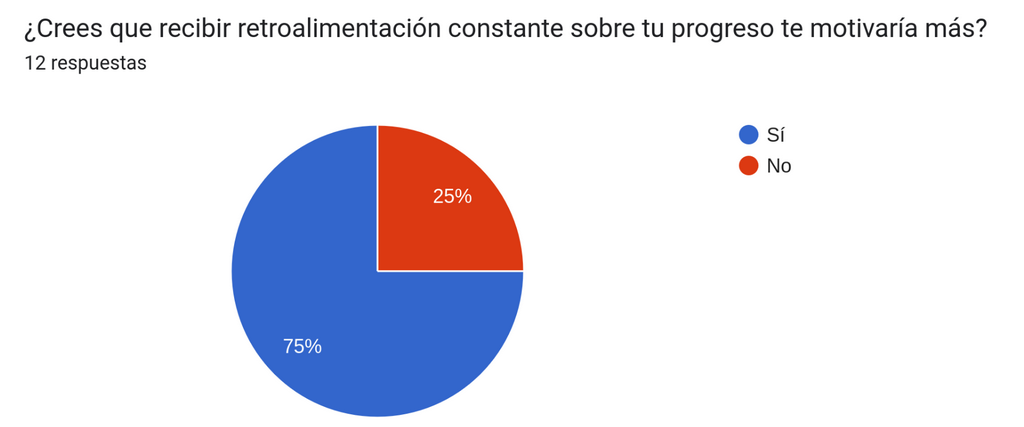
\includegraphics[width=1\textwidth]{Imagenes/Bitmap/ApendiceB/18.png}
          
          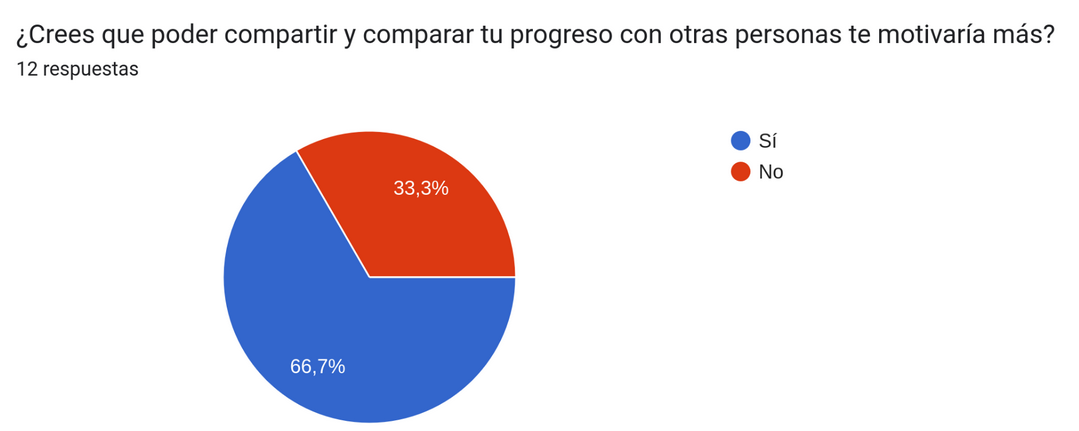
\includegraphics[width=1\textwidth]{Imagenes/Bitmap/ApendiceB/19.png}
          
          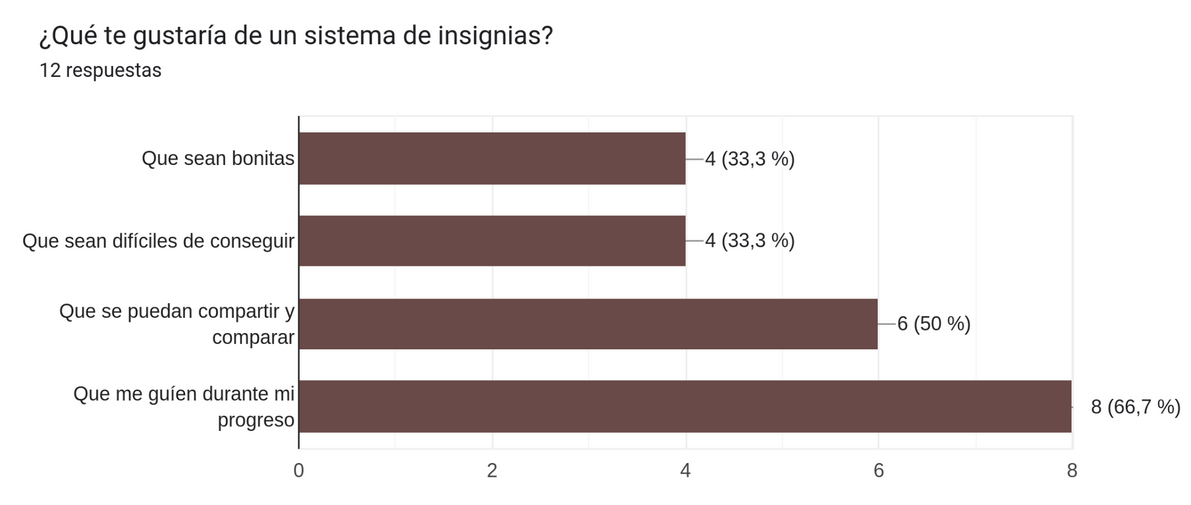
\includegraphics[width=1\textwidth]{Imagenes/Bitmap/ApendiceB/20.png}
          
          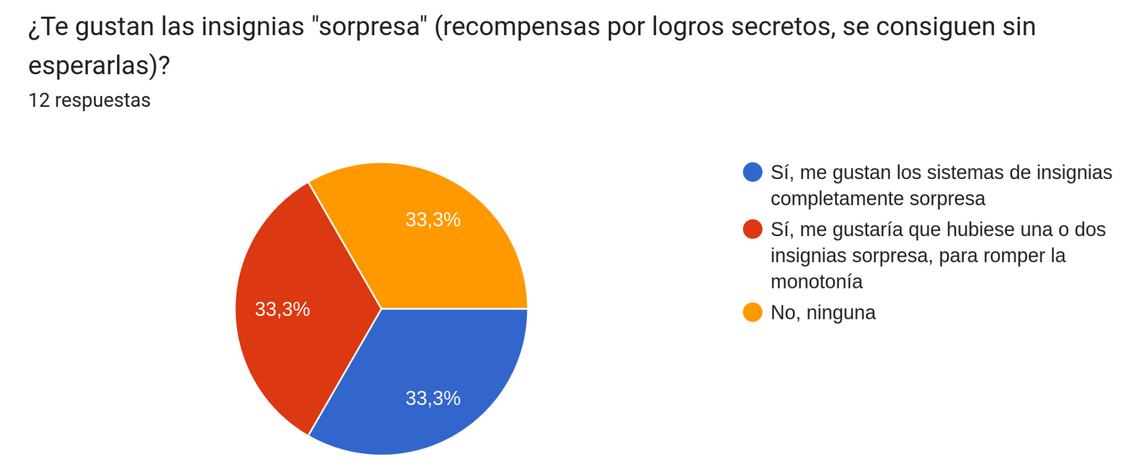
\includegraphics[width=1\textwidth]{Imagenes/Bitmap/ApendiceB/21.png}
          
          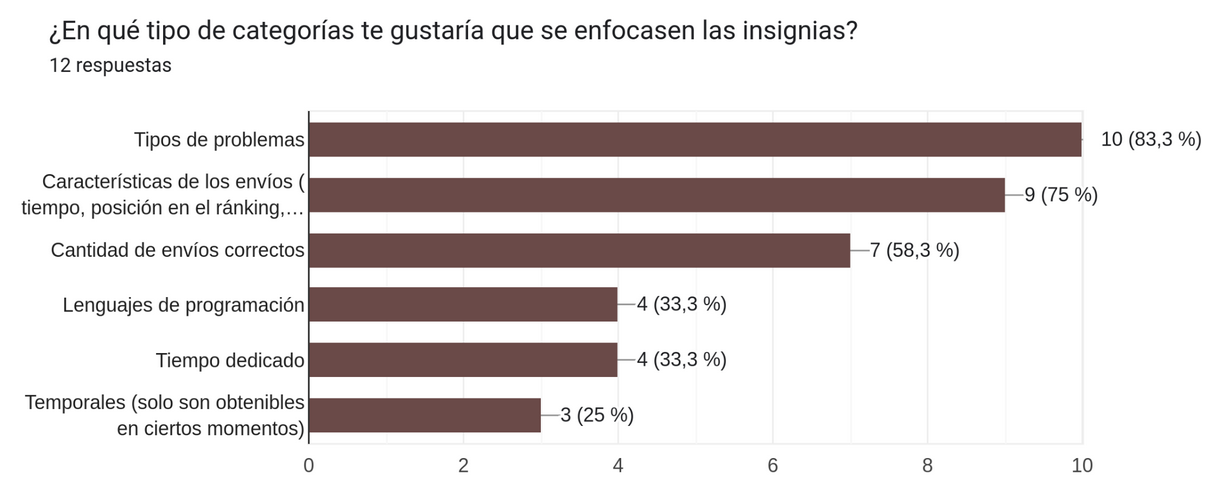
\includegraphics[width=1\textwidth]{Imagenes/Bitmap/ApendiceB/22.png}
          
          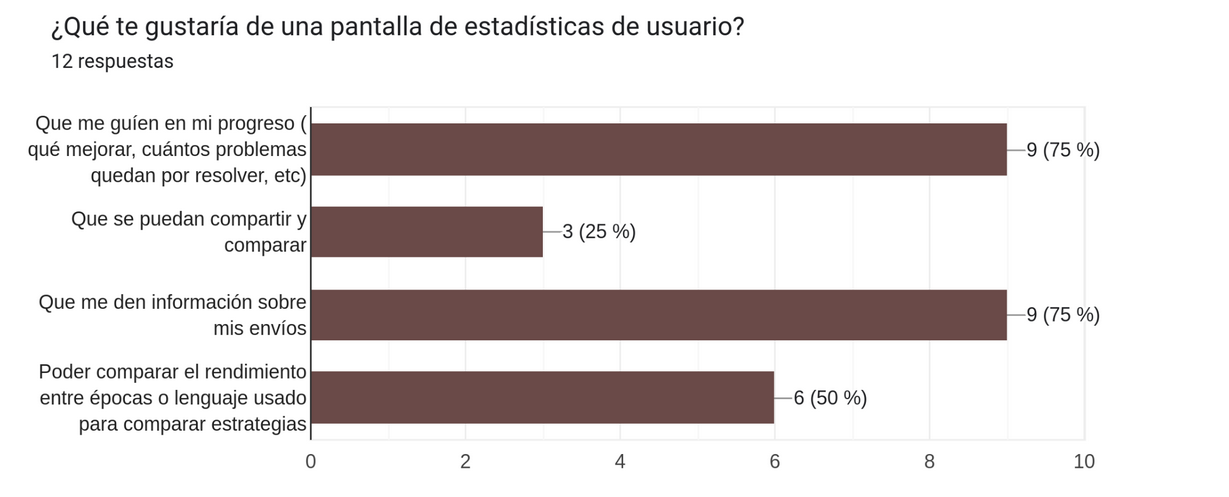
\includegraphics[width=1\textwidth]{Imagenes/Bitmap/ApendiceB/23.png}
          
          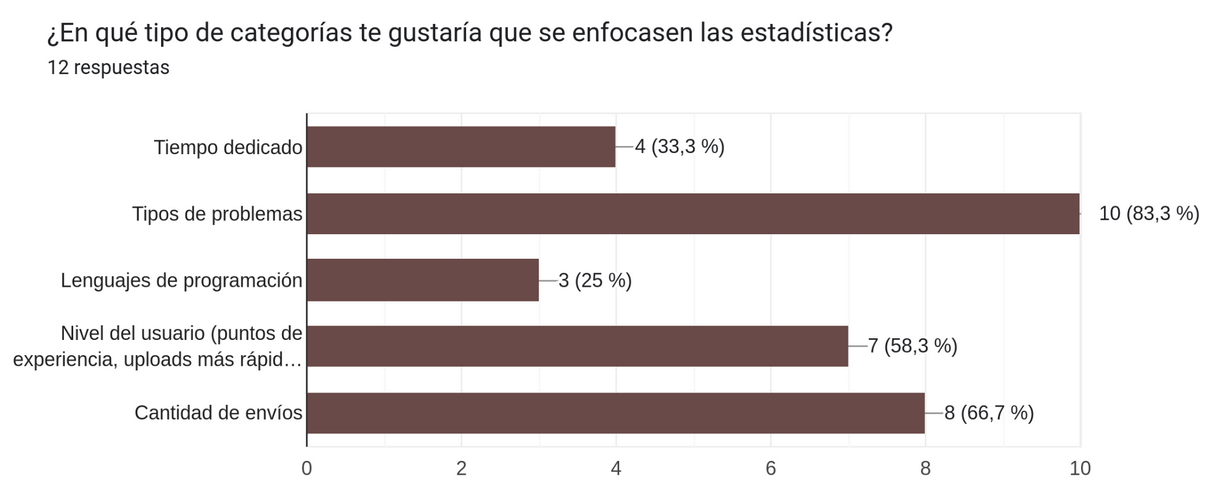
\includegraphics[width=1\textwidth]{Imagenes/Bitmap/ApendiceB/24.png}
          
          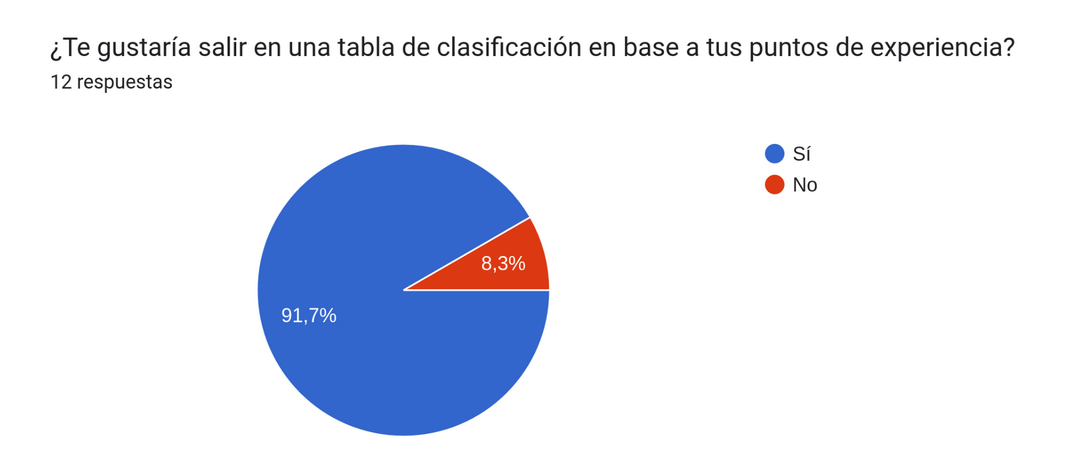
\includegraphics[width=1\textwidth]{Imagenes/Bitmap/ApendiceB/25.png}
          
          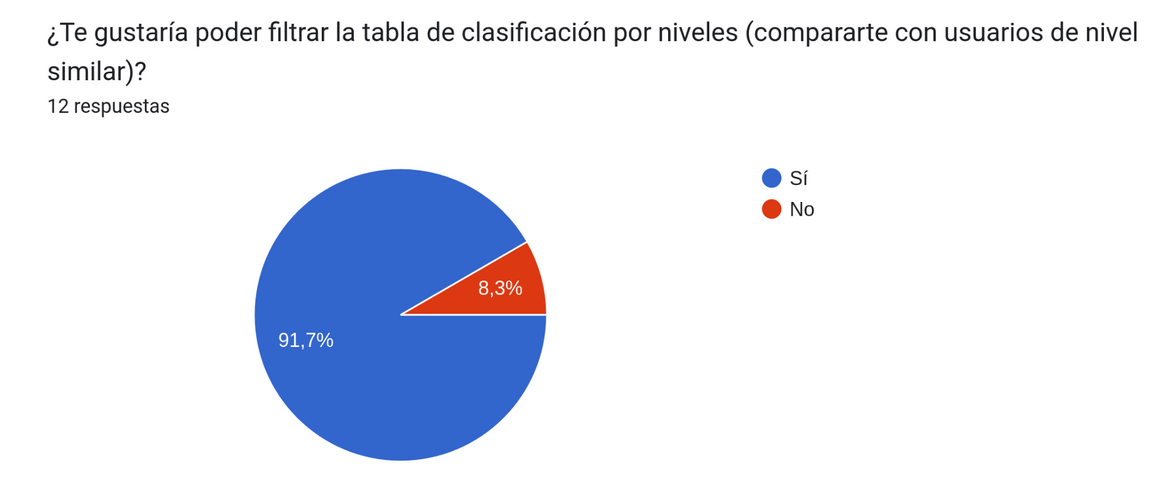
\includegraphics[width=1\textwidth]{Imagenes/Bitmap/ApendiceB/26.png}
          
          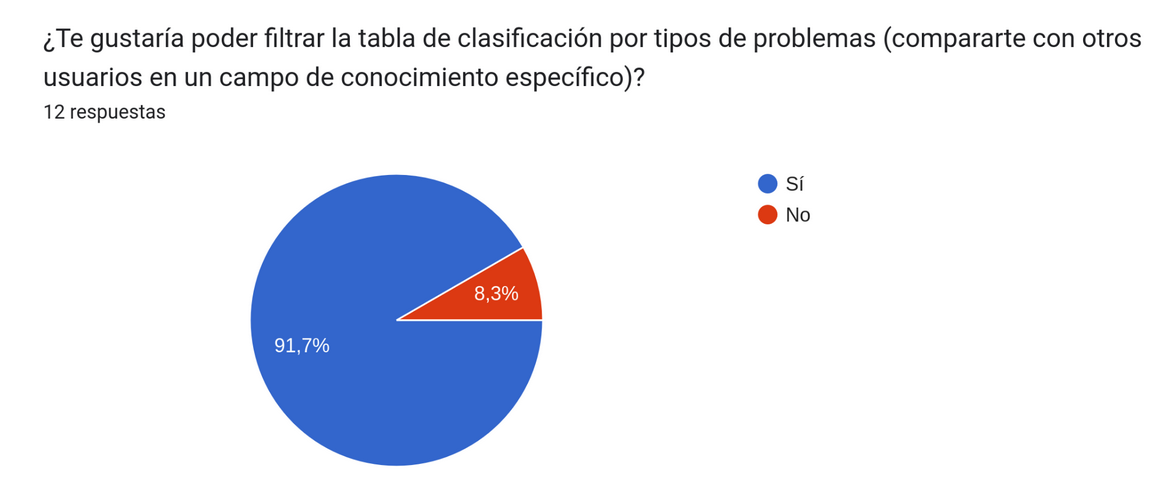
\includegraphics[width=1\textwidth]{Imagenes/Bitmap/ApendiceB/27.png}
          
\section{Información extra y retroalimentación}

          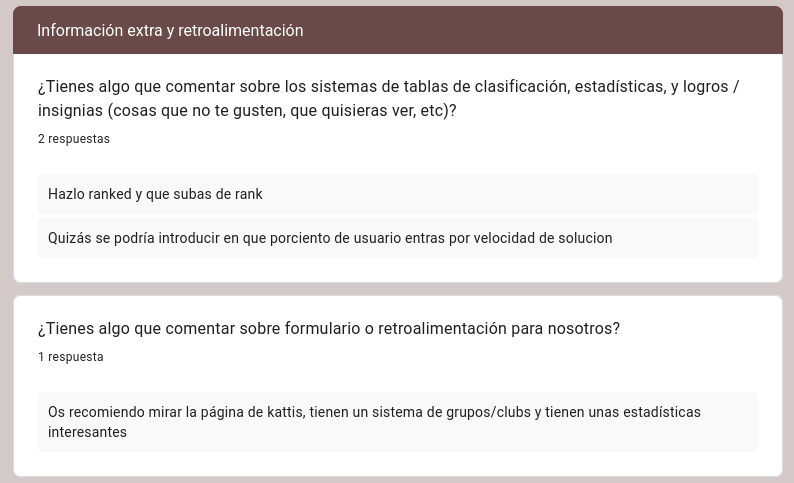
\includegraphics[width=1\textwidth]{Imagenes/Bitmap/ApendiceB/28.png}
          